\section{Limits involving infinity}\label{S:1.2.Infinity}

\begin{goals}
\item What does it mean to say that $\ds \lim_{x \to \infty} f(x) = L$ and $\ds \lim_{x \to a} f(x) = \infty$?
\item What is the connection between limits involving infinity and the asymptotes of a function?
\end{goals}

%--------------------------------------
% SUBSECTION INTRODUCTION
%--------------------------------------
\subsection{Introduction}

\begin{marginfigure}[2.25in]
\margingraphics{figures/2_8_Infty.eps}
\caption{The graph of $f(x) = \frac{1}{x}$.} \label{fig:2.8.Infty}
\end{marginfigure}

The concept of infinity\index{infinity}, denoted $\infty$, arises naturally in calculus, like it does in much of mathematics.  It is important to note from the outset that $\infty$ is a concept, but not a number itself.  Indeed, the notion of $\infty$ naturally invokes the idea of limits.  Consider, for example, the function $f(x) = \frac{1}{x}$, whose graph is pictured in Figure~\ref{fig:2.8.Infty}.

We note that $x = 0$ is not in the domain of $f$, so we may naturally wonder what happens as $x \to 0$.  As $x \to 0^+$, we observe that $f(x)$ \emph{increases without bound}.  That is, we can make the value of $f(x)$ as large as we like by taking $x$ closer and closer (but not equal) to $0$, while keeping $x > 0$.  This is a good way to think about what infinity represents:  a quantity is tending to infinity if there is no single number that the quantity is always less than. 

Recall that when we write $\ds \lim_{x \to a} f(x) = L$, this means that we can make $f(x)$ as close to $L$ as we'd like by taking $x$ sufficiently close (but not equal) to $a$.  We thus expand this notation and language to include the possibility that either $L$ or $a$ can be $\infty$.  For instance, for $f(x) = \frac{1}{x}$, we now write
$$\lim_{x \to 0^+} \frac{1}{x} = \infty,$$
by which we mean that we can make $\frac{1}{x}$ as large as we like by taking $x$ sufficiently close (but not equal) to $0$.  When we write the limit is equal to $\infty$ or $-\infty$, we call that limit an {\em infinite limit}.

Note that we are not saying the limit exists.  It doesn't since the function does not approach a single, unique real number as $x \to 0^+$.  We just give a special designation for a limit that does not exist because the function grows without bound in the positive or negative direction. 

In a similar way, we naturally write
$$\lim_{x \to \infty} \frac{1}{x} = 0,$$
since we can make $\frac{1}{x}$ as close to $0$ as we'd like by taking $x$ sufficiently large (i.e., by letting $x$ increase without bound).  This limit does exist because $0$ is a single, unique real number.

In general, we understand the notation $\ds \lim_{x \to a} f(x) = \infty$ to mean that we can make $f(x)$ as large as we'd like by taking $x$ sufficiently close (but not equal) to $a$, and the notation $\ds \lim_{x \to \infty} f(x) = L$ to mean that we can make $f(x)$ as close to $L$ as we'd like by taking $x$ sufficiently large.  This notation applies to left- and right-hand limits, plus we can also use limits involving $-\infty$.  For example, returning to Figure~\ref{fig:2.8.Infty} and $f(x) = \frac{1}{x}$, we can say that
$$\lim_{x \to 0^-} \frac{1}{x} = -\infty \ \ \mbox{and} \ \ \lim_{x \to -\infty} \frac{1}{x} = 0.$$
Finally, we write
$$\lim_{x \to \infty} f(x) = \infty$$
when we can make the value of $f(x)$ as large as we'd like by taking $x$ sufficiently large.  For example, $$\lim_{x \to \infty} x^2 = \infty.$$

\begin{marginfigure}[6cm]
\margingraphics{figs/1/1-2_PA.pdf}
\caption{The graph of $y = f(x)$.} \label{fig:1.2.PA1}
\end{marginfigure}

\begin{pa} \label{PA:1.2}
Using the graph of $f$ in Figure~\ref{fig:1.2.PA1}, evaluate the following, being sure to use any special designations if needed.

\begin{multicols}{2}
\ba
\item $\ds \lim_{x \to -\infty} f(x)$
\item $\ds \lim_{x \to -2^-} f(x)$
\item $\ds \lim_{x \to -2^+} f(x)$
\item $\ds \lim_{x \to -2} f(x)$
\item $\ds f(0)$
\item $\ds \lim_{x \to 0} f(x)$
\item $\ds \lim_{x \to 2^-} f(x)$
\item $\ds \lim_{x \to 2^+} f(x)$
\item $\ds \lim_{x \to 2} f(x)$
\item $\ds \lim_{x \to \infty} f(x)$
\ea
\end{multicols}
\end{pa} 

\afterpa

 % PREVIEW ACTIVITY

Note particularly that limits involving infinity identify \emph{vertical} and \emph{horizontal asymptotes} \index{asymptote} \index{asymptote!vertical} \index{asymptote!horizontal} of a function.  If $\ds \lim_{x \to a} f(x) = \infty$, then $x = a$ is a vertical asymptote of $f$, while if $\ds \lim_{x \to \infty} f(x) = L$, then $y = L$ is a horizontal asymptote of $f$.  Similar statements can be made using $-\infty$, as well as with left- and right-hand limits as $x \to a^-$ or $x \to a^+$.

%---------------------------------------
% SUBSECTION INFINITE LIMITS
%---------------------------------------
\subsection*{Infinite Limits}

We can easily determine if $\ds \lim_{x \to a} f(x)$ is an infinite limit by observing the graph of $f(x)$.  But what if we have no graph?  How do we determine if $\ds \lim_{x \to a} f(x)$ is an infinite limit or not?

In Section~\ref{S:1.1.Limits}, we learned the method of Direct Substitution to evaluate limits.  Now, we can use that method to determine if a limit is an infinite limit.  Certainly, if
\[ \lim_{x \to a} f(x) = f(a) = \pm \infty, \]
then we have an infinite limit.  However, we may also have an infinite limit if
\[ \lim_{x \to a} f(x) = f(a) = \frac{\mbox{a nonzero real number}}{0} \ . \]

\begin{marginfigure} % MARGIN FIGURE
\margingraphics{figs/1/figoneoverxsquared.pdf}
\caption{Graphing $f(x) = 1/x^2$ for values of $x$ near 0.}\label{fig:oneoverxsquared}
\end{marginfigure}

Consider $f(x) = 1/x^2$ as shown in Figure~\ref{fig:oneoverxsquared} and $\ds \lim_{x \to 0} f(x)$. Note that if evaluate $f(0)$, we have
\[ f(0) = \frac{1}{0^2} = \frac{1}{0}. \]
But also observe in the graph how, as $x$ approaches $0$ from both the left and the right, $f(x)$ grows without bound. So we can state that 
\[ \lim_{x \to 0} \frac{1}{x^2}=\infty.\]

Consider $f(x) = 1/x$ as shown in Figure~\ref{fig:2.8.Infty} one more time.  Again, if we evaluate $f(0)$, then we have
\[ f(0) = \frac{1}{0}, \]
but observing the graph, we see that the function grows without bound in different directions from the left and right.  Since that happens, we do not give a special designation to this limit and simply say that the limit as $x \to 0$ does not exist, i.e.,
\[ \lim_{x \to 0} \frac{1}{x} = \enskip \mbox{Does Not Exist.} \]

So we can determine if we have an infinite limit when by Direct Substitution, we have $f(a) = \frac{\mbox{a nonzero real number}}{0}$ and then comparing the individual left- and right-sided limits.  If they're the same, then we give the appropriate special designation.  If not, then we simply say the limit does not exist.

\begin{example} \label{Ex:1.2.Eg1}
Evaluate the possible infinite limit:  $\ds \lim_{x \to 1} \frac{1}{(x-1)^2}$.

\solution By Direct Substitution, we have
\[ \lim_{x \to 1} \frac{1}{(x-1)^2} = \frac{1}{(1-1)^2} = \frac{1}{0}, \]
so now we need to compare the one-sided limits
\[  \lim_{x \to 1^-} \frac{1}{(x-1)^2} \quad \mbox{and} \quad \lim_{x \to 1^+} \frac{1}{(x-1)^2}. \]
As $x \to 1^-$, the quantity $(x-1)^2 \to 0$ and is positive; therefore, $\ds \lim_{x \to 1^-} \frac{1}{(x-1)^2} = \infty$.  As $x \to 1^+$, the quantity $(x-1)^2 \to 0$ and is positive; therefore, $\ds \lim_{x \to 1^+} \frac{1}{(x-1)^2} = \infty$, and we can say that
\[ \lim_{x \to 1} \frac{1}{(x-1)^2} = \infty. \]
\end{example} % EXAMPLE

\begin{example} \label{Ex:1.2.Eg1}
Evaluate the possible infinite limit:  $\ds \lim_{x \to 1} \frac{1}{(x-1)^3}$.

\solution By Direct Substitution, we have
\[ \lim_{x \to 1} \frac{1}{(x-1)^3} = \frac{1}{(1-1)^3} = \frac{1}{0}, \]
so now we need to compare the one-sided limits
\[  \lim_{x \to 1^-} \frac{1}{(x-1)^3} \quad \mbox{and} \quad \lim_{x \to 1^+} \frac{1}{(x-1)^3}. \]
As $x \to 1^-$, the quantity $(x-1)^3 \to 0$ and is negative; therefore, $\ds \lim_{x \to 1^-} \frac{1}{(x-1)^3} = -\infty$.  As $x \to 1^+$, the quantity $(x-1)^3 \to 0$ and is positive; therefore, $\ds \lim_{x \to 1^+} \frac{1}{(x-1)^3} = \infty$, and we can say that
\[ \lim_{x \to 1} \frac{1}{(x-1)^2} = \enskip \mbox{Does not exist}. \]
\end{example} % EXAMPLE

\begin{activity} \label{A:1.2.1}  Evaluate the following infinite limits analytically.  
\ba
\item 
	\begin{enumerate*}[i)] 
	\item $\ds \lim_{x \to 2^+} \frac{1}{x-2} \quad$ 
	\item $\ds \lim_{x \to 2^-} \frac{1}{x-2} \quad$
	\item $\ds \lim_{x \to 2} \frac{1}{x-2}$ 
	\end{enumerate*}
	
\item 
	\begin{enumerate*}[i)] 
	\item $\ds \lim_{x \to 3^+} \frac{x+2}{(x-3)^3} \quad$ 
	\item $\ds \lim_{x \to 3^-} \frac{x+2}{(x-3)^3} \quad$
	\item $\ds \lim_{x \to 3} \frac{x+2}{(x-3)^3}$ 
	\end{enumerate*}
	
\item
	\begin{enumerate*}[i)] 
	\item $\ds \lim_{x \to 4^+} \frac{x-5}{(x-4)^2} \quad$ 
	\item $\ds \lim_{x \to 4^-} \frac{x-5}{(x-4)^2} \quad$
	\item $\ds \lim_{x \to 4} \frac{x-5}{(x-4)^2}$ 
	\end{enumerate*}
\ea
\end{activity}
\begin{smallhint}
\ba
	\item $(x^2 - 1)$ can be factored.
	\item Expand the expression $(2+x)^3$, and then combine like terms in the numerator.
	\item Try multiplying the given function by this fancy form of 1: $\frac{\sqrt{x+1} + 1}{\sqrt{x+1} + 1}$.
\ea
\end{smallhint}
\begin{bighint}
\ba
	\item $(x^2 - 1) = (x+1)(x-1)$.
	\item Expand the expression $(2+x)^3$ using the rule $(a+b)^3 = a^3 + 3a^2b + 3ab^2 + b^3$, and then combine like terms in the numerator.
	\item Try multiplying the given function by this fancy form of 1: $\frac{\sqrt{x+1} + 1}{\sqrt{x+1} + 1}$.  Expand and simplify the numerator, and then see what happens as $x \to 0$.
\ea
\end{bighint}
\begin{activitySolution}
Estimating the values of the limits with tables is straightforward and should suggest the exact values stated below.
\ba
	\item $\ds \lim_{x \to 1} \frac{x^2 - 1}{x-1} = \lim_{x \to 1} \frac{(x+1)(x-1)}{x-1} = \lim_{x \to 1} (x+1) = 2$. 
	\item $\ds \lim_{x \to 0} \frac{(2+x)^3 - 8}{x} = \lim_{x \to 0} \frac{8 + 12x + 6x^2 + x^3 - 8}{x} = \lim_{x \to 0} \frac{12x + 6x^2 + x^3}{x} =  \lim_{x \to 0} (12 + 6x + x^2) = 12$.
	\item $\ds \lim_{x \to 0} \frac{\sqrt{x+1} - 1}{x} = \lim_{x \to 0} \frac{\sqrt{x+1} - 1}{x} \cdot \frac{\sqrt{x+1} + 1}{\sqrt{x+1} + 1} = \lim_{x \to 0} \frac{x+1-1}{x(\sqrt{x+1}+1)} = \lim_{x \to 0} \frac{1}{\sqrt{x+1}+1} = \frac{1}{2}.$
\ea
\end{activitySolution}
\aftera
 % ACTIVITY

%-------------------------------------------
% SUBSECTION LIMITS AT INFINITY
%-------------------------------------------
\subsection{Limits at Infinity}

In precalculus classes, it is common to study the \emph{end behavior} of certain families of functions, by which we mean the behavior of a function as $x \to \infty$ and as $x \to -\infty$, or the limit of the function as $x \to \infty$ and as $x \to -\infty$.

For polynomial functions of the form 
\[ p(x) = a_n x^n + a_{n-1}x^{n-1} + \cdots a_1 x + a_0,\] 
the limit at infinity, or end behavior, depends on the sign of $a_n$ and whether the highest power $n$ is even or odd.  If $n$ is even and $a_n$ is positive, then $\ds \lim_{x \to \infty} p(x) = \infty$ and $\ds \lim_{x \to -\infty} p(x) = \infty$, as in the plot of $g$ in Figure~\ref{fig:1-2_Enda}.  If instead $a_n$ is negative, then $\ds \lim_{x \to \infty} p(x) = -\infty$ and $\ds \lim_{x \to -\infty} p(x) = -\infty$.  In the situation where $n$ is odd, then either $\ds \lim_{x \to \infty} p(x) = \infty$ and $\ds \lim_{x \to -\infty} p(x) = \infty$ (which occurs when $a_n$ is positive, as in the graph of $f$ in Figure~\ref{fig:1-2_Enda}), or $\ds \lim_{x \to \infty} p(x) = \infty$ and $\ds \lim_{x \to -\infty} p(x) = \infty$ (when $a_n$ is negative).

\begin{marginfigure}[-7cm] % MARGIN FIGURE
\margingraphics{figs/1/1-2_Enda.pdf}
\caption{The graphs of $f(x) = x^3 - 16x$ and $g(x) = x^4 - 16x^2-8$.}\label{fig:1-2_Enda}
\end{marginfigure}

\begin{marginfigure} % MARGIN FIGURE
\margingraphics{figs/1/1-2_Endb.pdf}
\caption{The graph of $f(x) =\sin(x)$.}\label{fig:1-2_Endb}
\end{marginfigure}

A function can fail to have a limit as $x \to \infty$.  For example, consider the plot of the sine function at right in Figure~\ref{fig:1-2_Endb}.  Because the function continues oscillating between $-1$ and $1$ as $x \to \infty$, we say that $\ds \lim_{x \to \infty} \sin(x)$ does not exist.

Finally, it is straightforward to analyze the behavior of any rational function as $x \to \infty$.  Consider, for example, the function 
\[ q(x) =  \frac{3x^2 - 4x + 5}{7x^2 + 9x - 10}. \]
Note that both $(3x^2 - 4x + 5) \to \infty$ as $x \to \infty$ and $(7x^2 + 9x - 10) \to \infty$ as $x \to \infty$.  Here we say that $\ds \lim_{x \to \infty} q(x)$ has indeterminate form $\ds \frac{\infty}{\infty}$, much like we did when we encountered limits of the form $\ds \frac{0}{0}$.  We can determine the value of this limit through a standard algebraic approach.  Multiplying the numerator and denominator each by $\frac{1}{x^2}$, we find that
\begin{eqnarray*}
\lim_{x \to \infty} q(x) & = & \lim_{x \to \infty} \frac{3x^2 - 4x + 5}{7x^2 + 9x - 10} \cdot \frac{\frac{1}{x^2}}{\frac{1}{x^2}} \\
& = & \lim_{x \to \infty} \frac{3 - 4\frac{1}{x} + 5\frac{1}{x^2}}{7 + 9\frac{1}{x} - 10\frac{1}{x^2}} \\
& = & \frac{3}{7}
\end{eqnarray*}
since $\frac{1}{x^2} \to 0$ and $\frac{1}{x} \to 0$ as $x \to \infty$.  This shows that the rational function $q$ has a horizontal asymptote at $y = \frac{3}{7}$.  A similar approach can be used to determine the limit of any rational function as $x \to \infty$.

\begin{activity} \label{A:1.2.2}  Evaluate $\ds \lim_{x \to \infty} f(x)$ and $\ds \lim_{x \to -\infty} f(x)$ for each of the rational functions.  
\begin{multicols}{2}
\ba
\item $\ds f(x) = \frac{4x}{20x+1}$
	
\item $\ds f(x) = \frac{3x^3 - 7}{x^4 + 5x^2}$
	
\item $\ds f(x) = \frac{4x^2 - 8}{8x^2 + 5x + 2}$

\item $\ds f(x) = \frac{-x^3 + 1}{2x + 8}$
\ea
\end{multicols}
\end{activity}
\begin{smallhint}
\ba
	\item $(x^2 - 1)$ can be factored.
	\item Expand the expression $(2+x)^3$, and then combine like terms in the numerator.
	\item Try multiplying the given function by this fancy form of 1: $\frac{\sqrt{x+1} + 1}{\sqrt{x+1} + 1}$.
\ea
\end{smallhint}
\begin{bighint}
\ba
	\item $(x^2 - 1) = (x+1)(x-1)$.
	\item Expand the expression $(2+x)^3$ using the rule $(a+b)^3 = a^3 + 3a^2b + 3ab^2 + b^3$, and then combine like terms in the numerator.
	\item Try multiplying the given function by this fancy form of 1: $\frac{\sqrt{x+1} + 1}{\sqrt{x+1} + 1}$.  Expand and simplify the numerator, and then see what happens as $x \to 0$.
\ea
\end{bighint}
\begin{activitySolution}
Estimating the values of the limits with tables is straightforward and should suggest the exact values stated below.
\ba
	\item $\ds \lim_{x \to 1} \frac{x^2 - 1}{x-1} = \lim_{x \to 1} \frac{(x+1)(x-1)}{x-1} = \lim_{x \to 1} (x+1) = 2$. 
	\item $\ds \lim_{x \to 0} \frac{(2+x)^3 - 8}{x} = \lim_{x \to 0} \frac{8 + 12x + 6x^2 + x^3 - 8}{x} = \lim_{x \to 0} \frac{12x + 6x^2 + x^3}{x} =  \lim_{x \to 0} (12 + 6x + x^2) = 12$.
	\item $\ds \lim_{x \to 0} \frac{\sqrt{x+1} - 1}{x} = \lim_{x \to 0} \frac{\sqrt{x+1} - 1}{x} \cdot \frac{\sqrt{x+1} + 1}{\sqrt{x+1} + 1} = \lim_{x \to 0} \frac{x+1-1}{x(\sqrt{x+1}+1)} = \lim_{x \to 0} \frac{1}{\sqrt{x+1}+1} = \frac{1}{2}.$
\ea
\end{activitySolution}
\aftera
 % ACTIVITY

%-------------
% SUMMARY
%-------------
\begin{summary}
\item With respect to the standard notation of a limit
\[ \lim_{x \to a} f(x) = L, \]
we can let express limits where either the value $a$ or $L$ grows without bound in the positive or negative directions.

\item The notions of {\em vertical and horizontal asymptotes} are directly connected to infinite limits and limits at infinity respectively.

\item The {\em end behavior} of a function is directly connected to limits at infinity.
\end{summary}

\clearpage

%--------------
% EXERCISES
%--------------
\begin{adjustwidth*}{}{-2.25in}
\textbf{{\large Exercises}}
\setlength{\columnsep}{25pt}
\begin{multicols*}{2}
\noindent Terms and Concepts \small

\begin{enumerate}[1)]
\item {T/F: If $\ds \lim_{x\to 5} f(x) = \infty$, then we are implicitly stating that the limit exists.}
\item {T/F: If $\ds \lim_{x\to \infty} f(x) = 5$, then we are implicitly stating that the limit exists.}
\item {T/F: If $\ds \lim_{x\to 1^-} f(x) = -\infty$, then $\ds \lim_{x\to 1^+} f(x) = \infty$}
\item {T/F: If $\ds \lim_{x\to 5} f(x) = \infty$, then $f$ has a vertical asymptote at $x=5$.}
\item {T/F: $\infty/0$ is not an indeterminate form.}
\item {Construct a function with a vertical asymptote at $x=5$ and a horizontal asymptote at $y=5$.}
%\item {Let $\ds \lim_{x\to 7} f(x) = \infty$. Explain how we know that $f$ is/is not continuous at $x=7$.}
\end{enumerate} 

\noindent {\normalsize Problems\\} \small

\noindent In exercises 7--12, evaluate each limit using the given graph of $f(x)$.

\begin{enumerate}[1),resume]
\item 
{$\ds f(x) = \frac{1}{(x+1)^2}$
\begin{enumerate}
\item		$\ds \lim_{x\to -1^-} f(x)$
\item		$\ds \lim_{x\to -1^+} f(x)$
\end{enumerate}

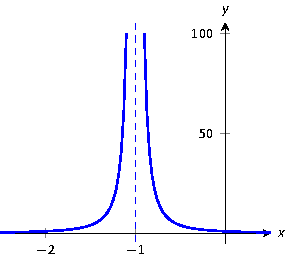
\includegraphics[scale=.8]{figures/fig01_06_ex_09}
}

\item
{$\ds f(x) = \frac{1}{(x-3)(x-5)^2}$.

\begin{minipage}[t]{.5\linewidth}
\begin{enumerate}
\item		$\ds \lim_{x\to 3^-} f(x)$
\item		$\ds \lim_{x\to 3^+} f(x)$
\item		$\ds \lim_{x\to 3} f(x)$
\end{enumerate}
\end{minipage}
\begin{minipage}[t]{.5\linewidth}
\begin{enumerate}\addtocounter{enumii}{3}
\item		$\ds \lim_{x\to 5^-} f(x)$
\item		$\ds \lim_{x\to 5^+} f(x)$
\item		$\ds \lim_{x\to 5} f(x)$
\end{enumerate}
\end{minipage}

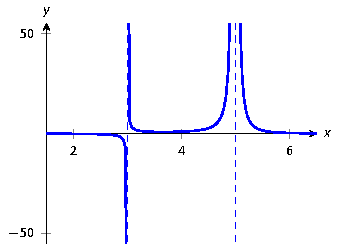
\includegraphics[scale=.8]{figures/fig01_06_ex_10}
}

\item
{$\ds f(x) = \frac{1}{e^x+1}$

\begin{minipage}[t]{.5\linewidth}
\begin{enumerate}
\item		$\ds \lim_{x\to -\infty} f(x)$
\item		$\ds \lim_{x\to \infty} f(x)$
\end{enumerate}
\end{minipage}
\begin{minipage}[t]{.5\linewidth}
\begin{enumerate}\addtocounter{enumii}{2}
\item		$\ds \lim_{x\to 0^-} f(x)$
\item		$\ds \lim_{x\to 0^+} f(x)$
\end{enumerate}
\end{minipage}

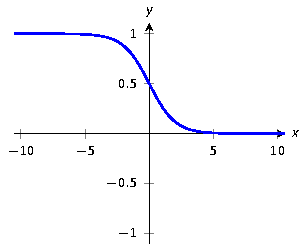
\includegraphics[scale=.8]{figures/fig01_06_ex_11}
}

\item
{$\ds f(x) = x^2\sin (\pi x)$

\begin{enumerate}
\item		$\ds \lim_{x\to -\infty} f(x)$
\item		$\ds \lim_{x\to \infty} f(x)$
\end{enumerate}

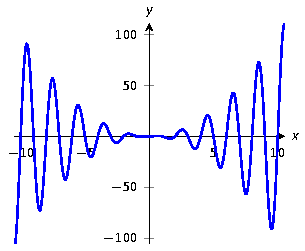
\includegraphics[scale=.8]{figures/fig01_06_ex_12}
}

\item
{$\ds f(x) = \cos (x)$

\begin{enumerate}
\item		$\ds \lim_{x\to -\infty} f(x)$
\item		$\ds \lim_{x\to \infty} f(x)$
\end{enumerate}

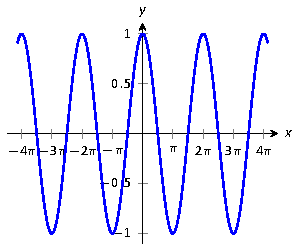
\includegraphics[scale=.8]{figures/fig01_06_ex_13}
}

\item
{$\ds f(x) = 2^x+10$
\begin{enumerate}
\item		$\ds \lim_{x\to -\infty} f(x)$
\item		$\ds \lim_{x\to \infty} f(x)$
\end{enumerate}

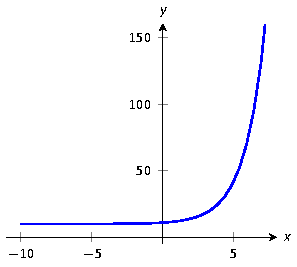
\includegraphics[scale=.8]{figures/fig01_06_ex_40}
}

\end{enumerate}

\vspace{.5cm}

%------------------------------------------
% END OF EXERCISES ON FIRST PAGE
%------------------------------------------
\end{multicols*}
\end{adjustwidth*}

\clearpage

\begin{adjustwidth*}{}{-2.25in}
\setlength{\columnsep}{25pt}
\begin{multicols*}{2}\small

In exercises 13--23, evaluate the limit.

\begin{multicols}{2}
\begin{enumerate}[1),start=13]
\item {$\ds \lim_{x \to -3^+} \frac{x-2}{x+3}$}
\item {$\ds \lim_{x \to 5^-} \frac{4}{x-5}$}
\item {$\ds \lim_{x \to 1} \frac{3-x}{(x-1)^2}$}
\item {$\ds \lim_{x \to \pi^-} \cot(x)$}
\item {$\ds \lim_{x\to\infty} \frac{x^3+2x^2+1}{5-x}$}
\item {$\ds \lim_{x\to-\infty} \frac{x^3+2x^2+1}{x^2-5}$}
\item {$\ds \lim_{x\to-\infty} \frac{x^3+2x^2+1}{5-x^2}$}
\item {$\ds \lim_{x \to \infty} \left( x - \sqrt{x} \right)$}
\item $\ds \lim_{x \to \infty} \frac{x+2}{\sqrt{9x^2 + 8}}$
\item $\ds \lim_{x \to -\infty} \frac{\sin^2(x)}{x^2}$
\item $\ds \lim_{x \to -\infty} \left( x^4 + x^5 \right)$
\end{enumerate}
\end{multicols}

\vspace{.5cm}

%---------------------------------------------
% END OF EXERCISES ON SECOND PAGE
%---------------------------------------------
\end{multicols*}
\end{adjustwidth*}
\afterexercises 

\cleardoublepage